\section{Theorie}
\label{sec:Theorie}

Mit der Phase eines Stoffes wird ein räumlich abgegrenzter Bereich in einem abgeschlossenen System beschrieben,
in dem sich der Stoff in einem physikalisch homogenen Zustand befindet. 
Darunter gelten unter anderem die Aggregatzustände: fest, flüssig und gasförmig.

In einem sogenannten Phasendiagramm (siehe Abbildung \ref{fig:phasendiagramm}) besitzt ein System
innerhalb eines abgegrenzten Bereichs zwei Freiheitsgrade, den Druck $p$ und die Temperatur $T$.
Das heißt, dass diese ohne Phasenänderung variiert werden können, solange keine Grenzlinie überschritten wird.
\begin{figure} 
    \centering
    \includegraphics[width=12cm] {pictures/phasendiagramm.pdf}  
    \caption{Qualitatives Phasendiagramm von Wasser. \cite[1]{v203}}
    \label{fig:phasendiagramm}
\end{figure}

Zur Untersuchung des Übergangs von flüssig zu gasförmig, wird die Grenzlinie zwischen dem
Tripelpunkt (TP.) und den kritischen Punkt (K.P.) betrachtet, der sogenannten \textit{Dampfdruckkurve}.
An dem Tripelpunkt liegen alle drei Phasen gleichzeitig, während entlang der Kurve bis zum
kritischen Punkt die flüssige und gasförmige Phase koexistieren.

Die Form dieser Dampfdruckkurve ist durch einen temperaturabhängigen Parameter festgelegt, 
der molaren \textit{Verdampfungswärme} $L$. 
Sie ist eine stoffspezifische Größe und gibt an, wie viel Wärmeenergie nötig ist, 
um ein Mol einer Flüssigkeit isotherm und isobar zu verdampfen.
Alle sich im System befindenden Teilchen haben dabei eine nach der Maxwellschen Geschwindigkeitsverteilung
vorgegebene Geschwindigkeit. 
Teilchen mit einer ausreichend hohen Geschwindigkeit können demnach die flüssige Phase verlassen und in die
gasförmige übergehen, nachdem sie die molekularen Bindungskräfte überwunden haben.
Die dazu nötige Energie muss entweder von außen hinzugefügt werden oder dem Wasser entzogen werden,
wodurch dieses abkühlt. 
Da die Teilchen in der gasförmigen Phase ebenfalls nach Maxwell verteilte Geschwindigkeiten haben, 
erfolgt dieser Prozess auch umgekehrt. 
Die Verdampfungswärme wird also bei der Kondensation wieder freigesetzt.

Nach einiger Zeit stellt sich ein Gleichgewicht zwischen Verdampfung und Kondensation ein. 
Der Druck, der dann herscht, wird \textit{Sättigungsdampfdruck} genannt.
Da dieser Druck nicht vom Volumen des Gasraumes abhängt, kann dieser nicht mithilfe der
\textit{idealen~Gasgleichung} 
\begin{equation}
    pV = RT \, , \: \text{mit der allgemeinen Gaskonstante} \: R \approx \qty{8.314}{\joule\per\mol\per\kelvin} \, ,
    \label{eq:idgasgleichung} 
\end{equation}
berechnet werden.

Zur Berechnung der Dampfdruckkurve wird dagegen der Kreisprozess der Verdampfung und Kondensation von Wasser
in Abbildung \ref{fig:kreisprozess} betrachtet.
\begin{figure} 
    \centering
    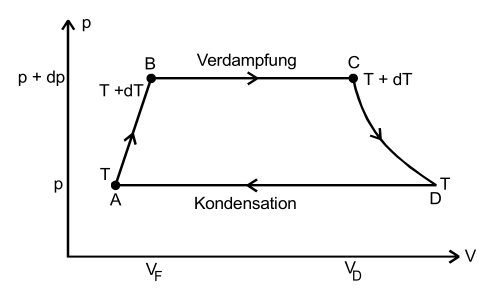
\includegraphics[width=12cm] {pictures/kreisprozess.pdf}  
    \caption{Kreisprozess von Wasser im $p$-$V$-Diagramm. \cite[3]{v203}}
    \label{fig:kreisprozess}
\end{figure}

Zunächst wird ein Mol einer Flüssigkeit um eine Temperatur $\dif{T}$ erhitzt, 
wobei sich der Druck um $\dif{p}$ erhöht und das Volumen auf $V_{\text{F}}$ ansteigt (A $\to$ B). 

Nach Zufuhr der Verdampfungswärme geht die Flüssigkeit isobar und isotherm in ein Gas über.
Das Volumen dehnt sich dabei von $V_{\text{F}}$ auf $V_{\text{D}}$ aus (B $\to$ C). 

Anschließend kühlt sich der Dampf wiederauf die Ursprungstemperatur $T$ ab 
und hat dann auch wieder den Ursprungsdruck $p$ (C $\to$ D).

Bei der nun isobar und isotherm erfolgenden Kondensation wird die Verdampfungswärme wieder freigesetzt (D $\to$ A).

Werden alle Wärmeenergien der vier Vorgänge addiert und mit der insgesamt verrichteten Arbeit gleichgesetzt,
so ergibt sich die Gleichung
\begin{equation}
    (C_\text{F} - (C_\text{D}) \dif{T} + \dif{L} = (V_\text{D} - V_\text{F}) \dif{p} \, .
\end{equation}

$C_\text{F}$ und $(C_\text{D}$ Sind dabei die Molwärmen im flüssigen beziehungsweise gasförmigen Zustand.
$\dif{L}$ beschreibt die Differenz der nötigen Verdampfungswärmen, da diese bei höheren Temperaturen sinkt.
Da hier ein reversibler Kreisprozess vorliegt, gilt nach dem Zweiten Hauptsatz der Thermodynamik für 
die Summe der reduzierten Wärmemengen
\begin{equation}
    \sum_{i} \frac{Q_{i}}{T_{i}} = 
    \frac {C_{F}\dif{T}} {T} + \frac {L+\dif{L}} {T+\dif{T}} - \frac {C_{D}\dif{T}} {T}-\frac{L}{T} =
    0 \, .
\end{equation}

